\begin{frame}
    \begin{block}{Synchronizacja pomiaru przesunięć}
        Pomiary wybranych odległości w przedziale $[0,1]$. Wykres po lewej - dane przed normalizacją do punktu $0$, natomiast prawy po normalizacji, okrojony do interesującego przedziału. Prosta $y=x$ wskazuje oczekiwane wyniki. Na prawym wykresie dodatkowa prosta przedstawia przybliżony współczynnik skalowania odległości.
    \end{block}
    \begin{figure}
        \centering
        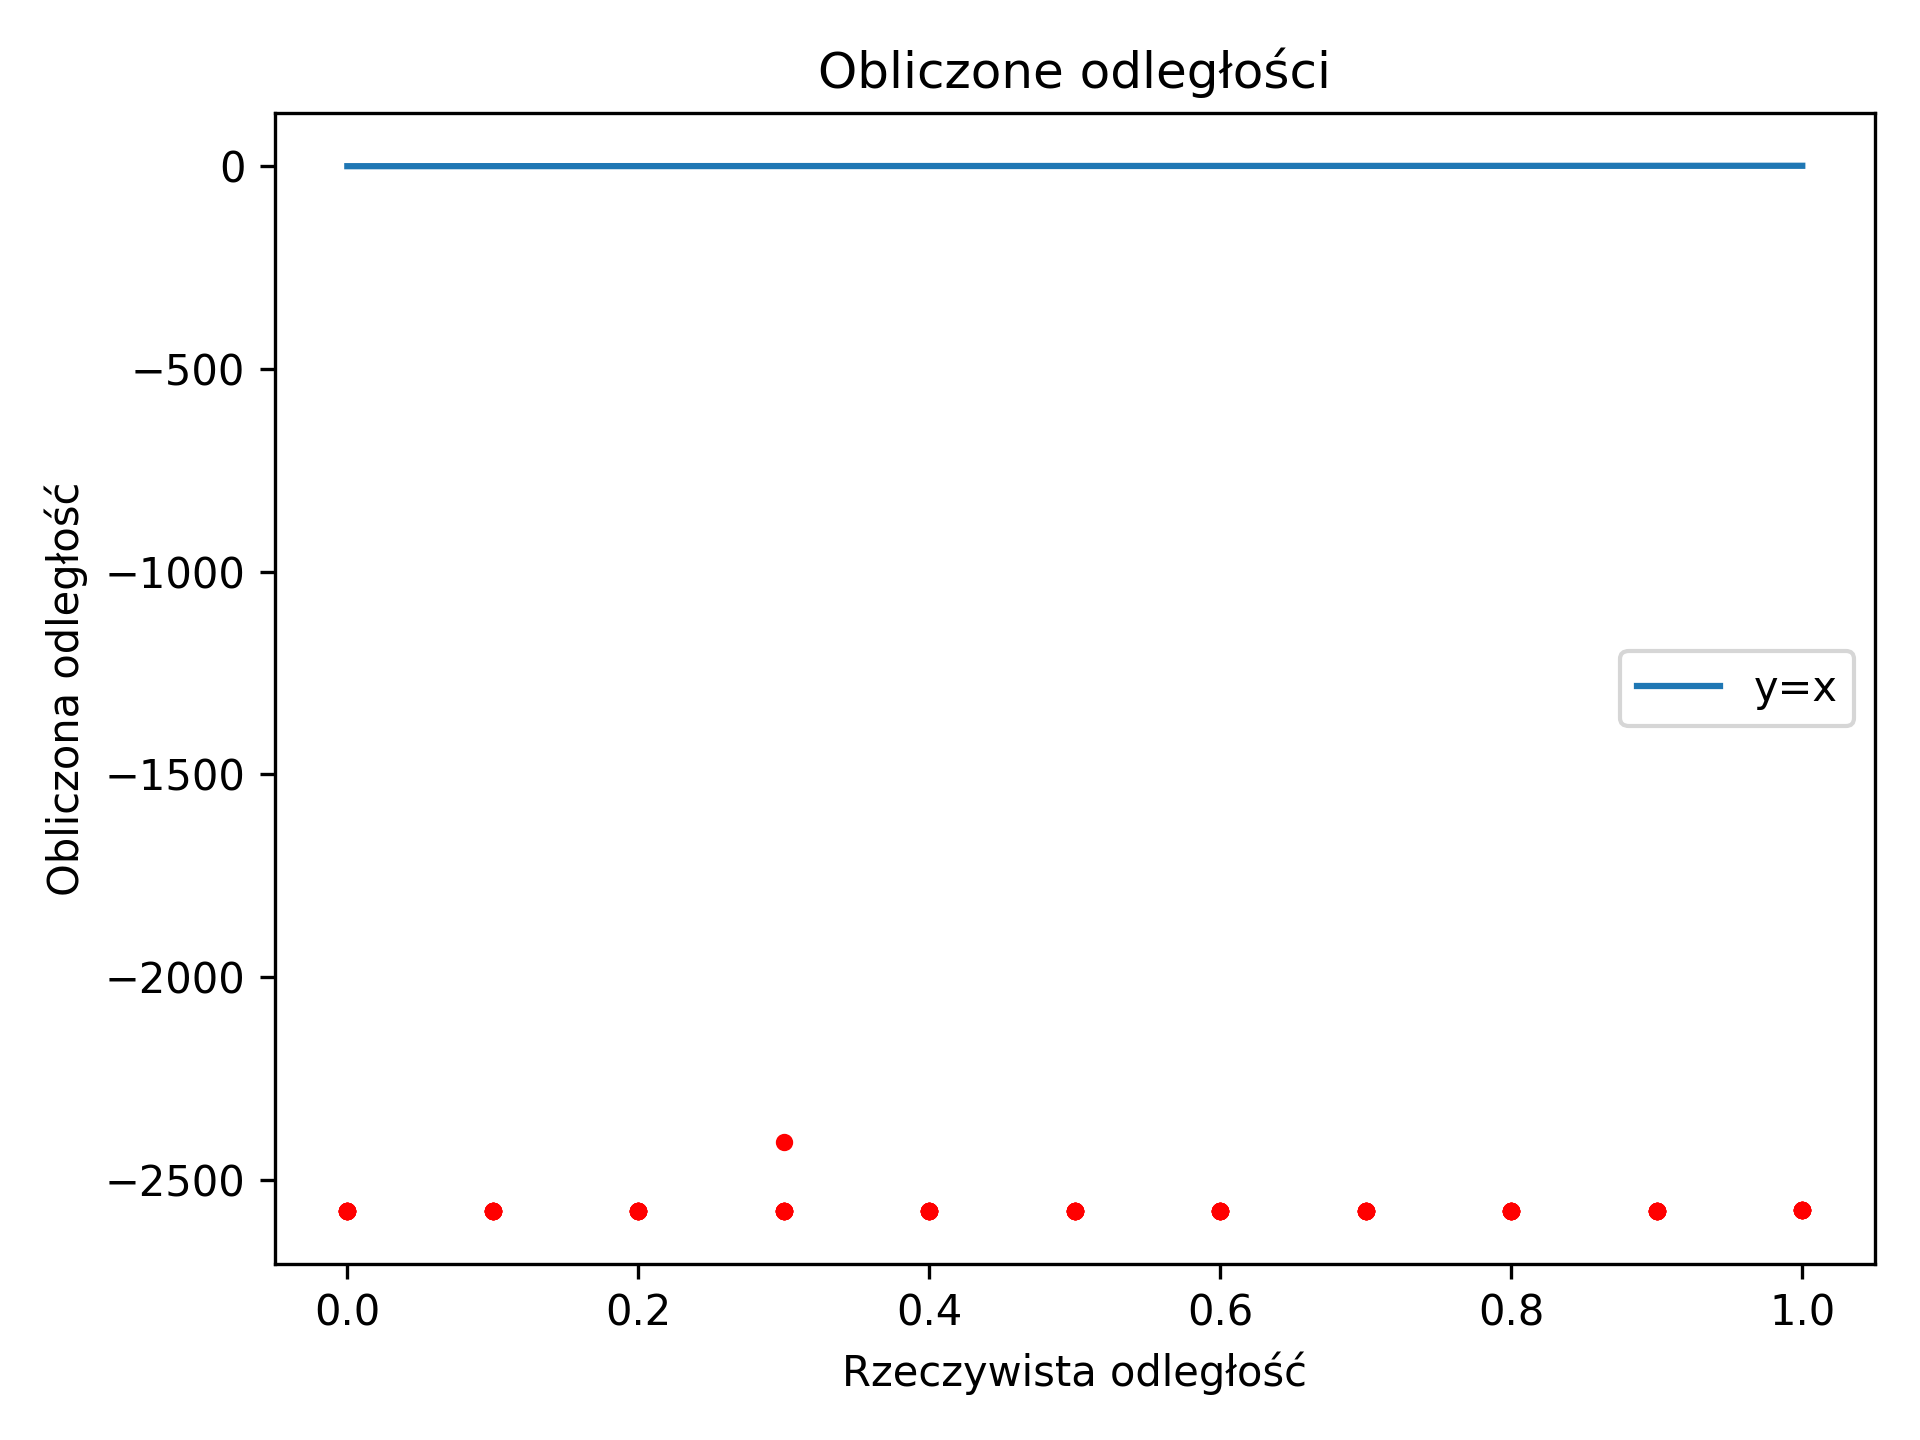
\includegraphics[width=0.49\textwidth]{../pics/time_deltas_dist/dists.png}
        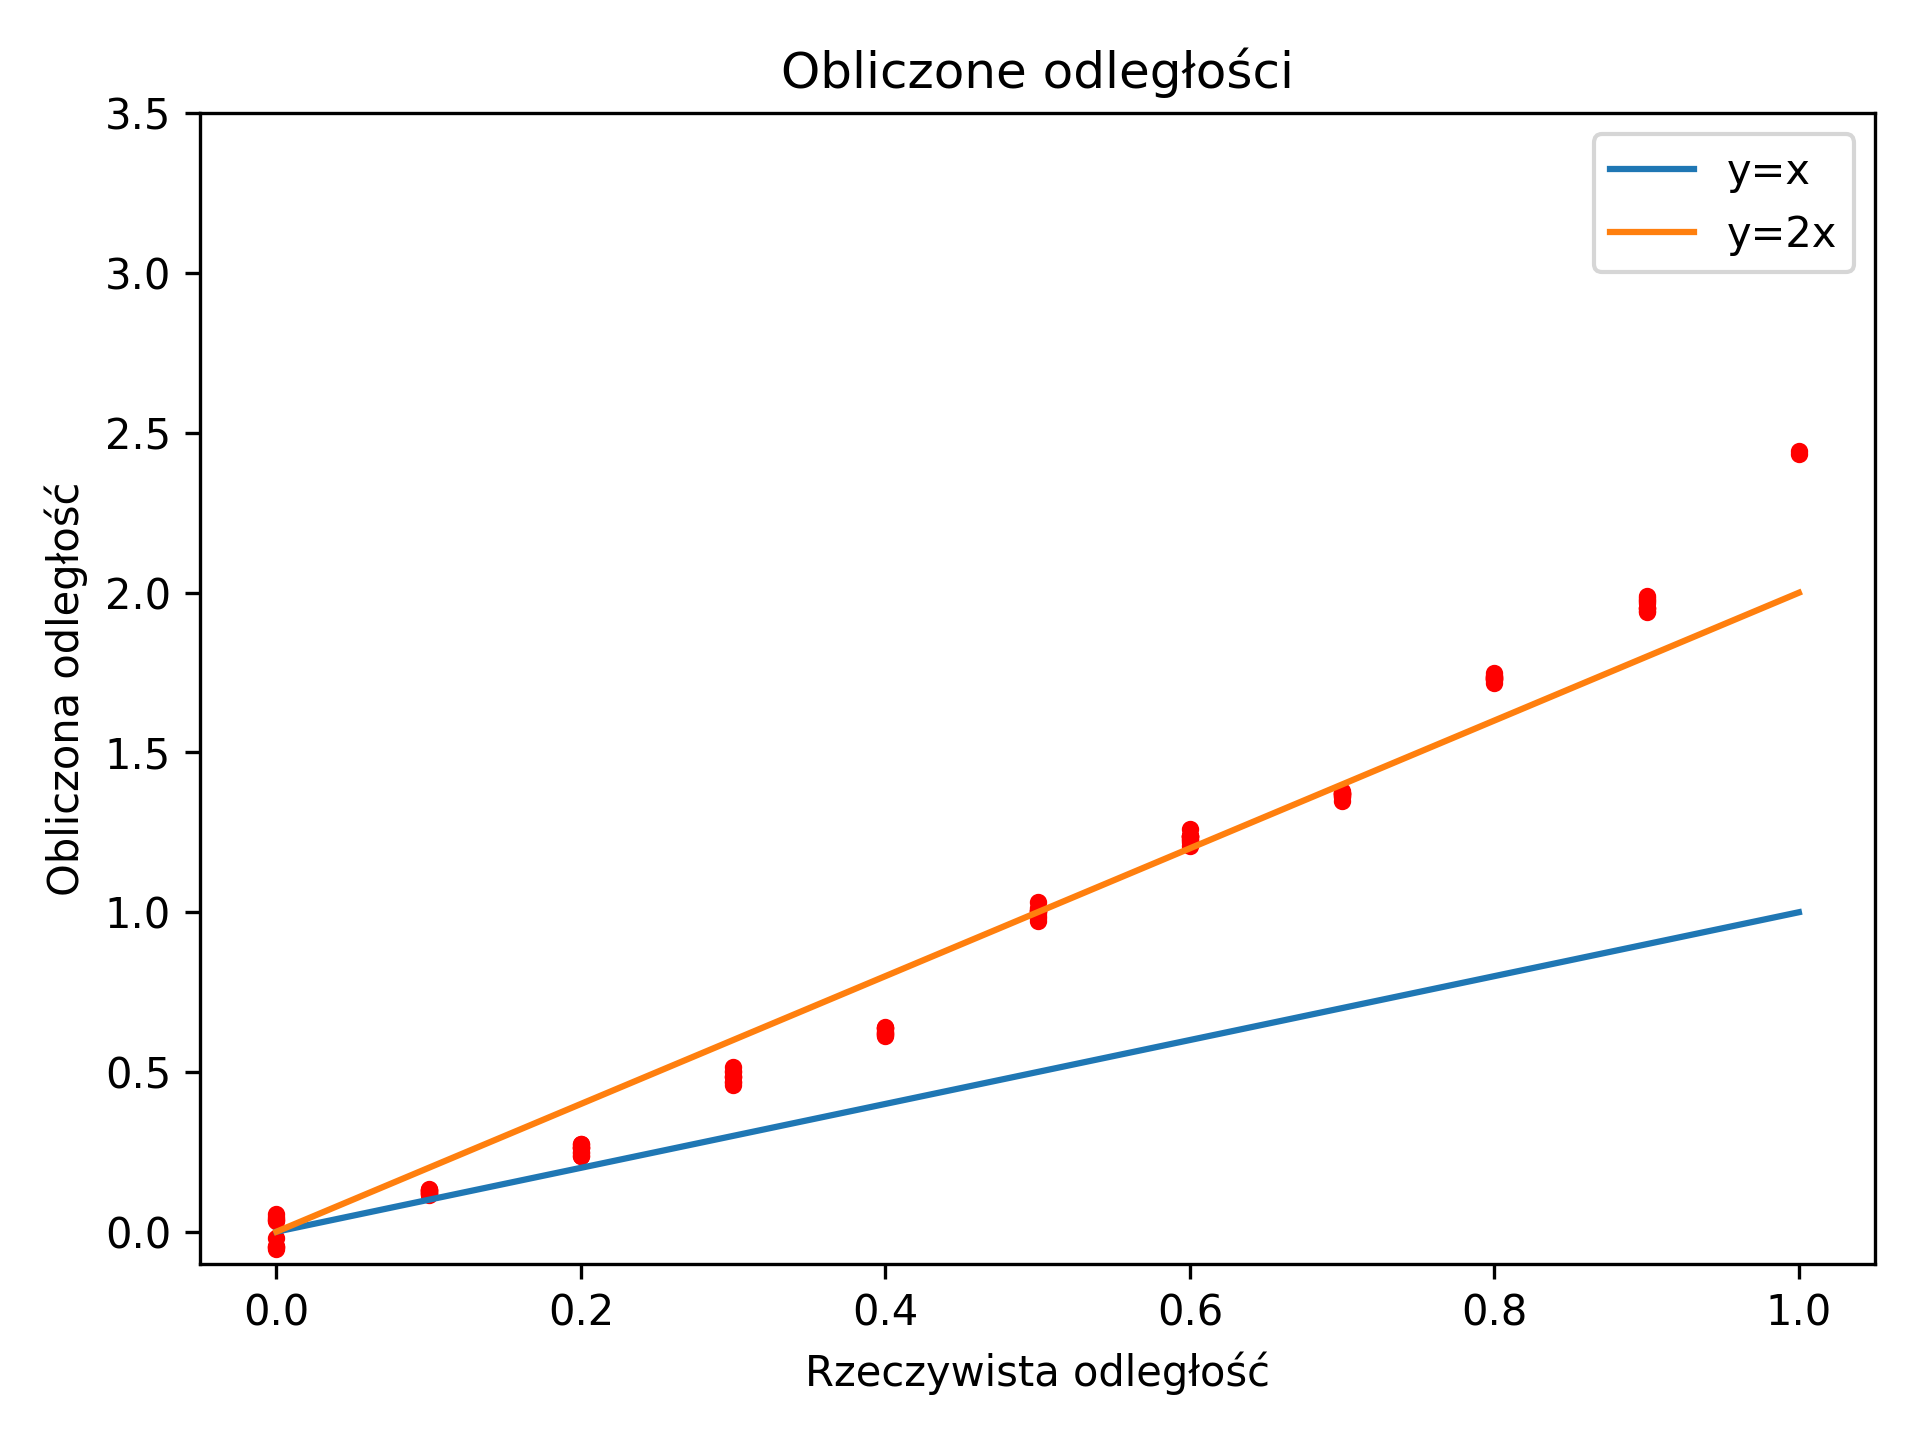
\includegraphics[width=0.49\textwidth]{../pics/time_deltas_dist/dists_close.png}
    \end{figure}
\end{frame}